\subsection{NOR}
    The NOR gate, short for NOT-OR, can be obtained by connecting an OR gate and a NOT gate in series, as shown in Figure \ref{fig:NOR_gate}. \\
    Its operation can be algebraically represented as $\text{NOR}(A, B) = \overline{A + B}$, where $A$ and $B$ are the input signals.
    When all inputs are low (0), all the transistors in the OR part are off, resulting in a low output (0) for the OR operation. 
    The NOT gate then inverts this low output to a high final output (1).
    This behavior is consistent with the NOR gate's truth table shown in Table \ref{tab:NOR_table}. \\
    The symbol for the NOR gate is shown in Figure \ref{fig:NOR_sym}.

    \begin{figure}[H]   
        \begin{minipage}{0.5\textwidth}
            \centering
            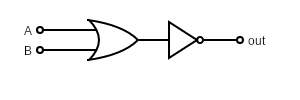
\includegraphics[width=1.1\textwidth]{figures/circuits/NOR.png}
            \captionof{figure}{NOR gate.} 
            \label{fig:NOR_gate} 
        \end{minipage}
        \begin{minipage}{0.5\textwidth}
            \centering
            \captionof{table}{NOR truth table.}
            \begin{tabular}{|c|c|c|}
                \hline
                Input A & Input B & Output \\
                \hline
                0 & 0 & 1 \\
                0 & 1 & 0 \\
                1 & 0 & 0 \\
                1 & 1 & 0 \\
                \hline
            \end{tabular}
            \label{tab:NOR_table}
        \end{minipage}
	\end{figure}

	\begin{figure}[H]
	    \centering
	    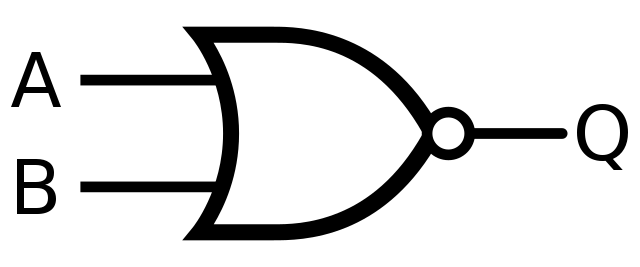
\includegraphics[width=0.3\textwidth]{figures/symbols/NOR.png}
	    \caption{NOR symbol.}
	    \label{fig:NOR_sym} 
	\end{figure}
